\chapter{Apache Kafka nell’Integrazione Aziendale}

% \section{L'evoluzione delle architetture di integrazione}
\section{Obiettivi aziendali}

Per soddisfare le richieste clientelari ed essere sempre competitiva e all'avanguardia, una priorità di Sync Lab sono le esplorazioni tecnologiche e di prodotto anche tramite l'utilizzo di percorsi di \stage\ insieme ai laureandi, come quanto accaduto nella mia esperienza.
Questi percorsi consentono all'azienda non solo di testare l'utilizzo di nuovi \software\ ma anche di conoscere e mettere alla prova le capacità del laureando in vista di una potenziale assunzione al termine dello \stage.
% Introduzione al motivo aziendale per cui è nato questo percorso di stage: la propensione odierna alle architetture a microservizi, la gestione di grandi flussi di dati in modo efficiente ed eff1icace, una richiesta di un sistema innovativo da parte della clientela.3
\begin{figure}[h]
  \begin{center}
    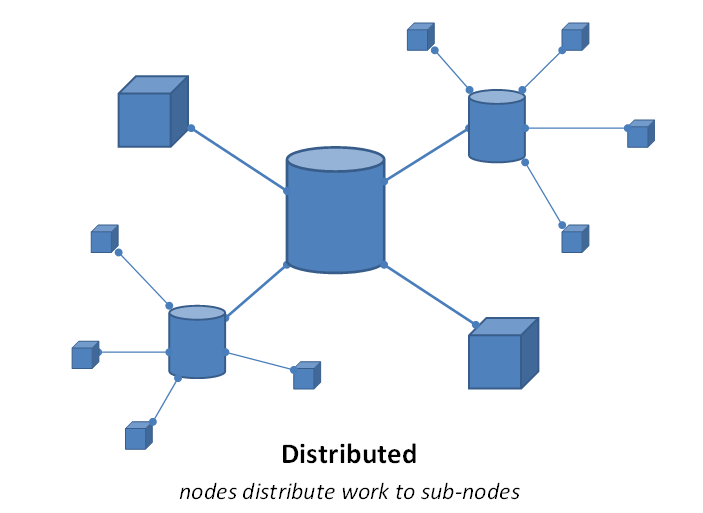
\includegraphics[width=0.6\textwidth]{images/distributed.png}
    \caption{Illustrazione di un sistema distribuito}
    \captionsetup{aboveskip=2pt}
    \caption*{\begin{footnotesize}\textit{Fonte:} \url{https://www.delphitools.info/DWSH/}\end{footnotesize}}
  \end{center}
\end{figure}

Nel settore dell'\gls{g_eai}, l'evoluzione tecnologica è diretta verso soluzioni sempre più distribuite e con un flusso di dati in continuo aumento.
Uno degli obiettivi specifici nell'area \sacr{eai} di Sync Lab è pertanto quello di trovare un \software\ o tecnologia in grado di soddisfare i bisogni dei clienti di gestire un flusso di dati di dimensioni molto maggiori a quelle attuali, tramite architetture a messaggio che utilizzano servizi distribuiti.

% \section{L’evoluzione delle architetture di integrazione}
%
% % Introduzione al motivo aziendale per cui è nato questo percorso di stage: la propensione odierna alle architetture a microservizi, la gestione di grandi flussi di dati in modo efficiente ed eff1icace, una richiesta di un sistema innovativo da parte della clientela.3
% L'evoluzione del settore dell'\textit{Enterprise Application Integration} verso soluzioni sempre più distribuite e con un flusso di dati in continuo aumento ha sviluppato nei clienti (e di conseguenza nell'azienda) un interesse verso il prodotto Apache Kafka.
% Il software ha dimostrato negli anni recenti un notevole successo in diversi campi; l'azienda ha interesse nel testare le capacità di Kafka nel soddisfare le esigenze dell'integrazione aziendale.
%
% \bigskip
% \begin{figure}[h]
%   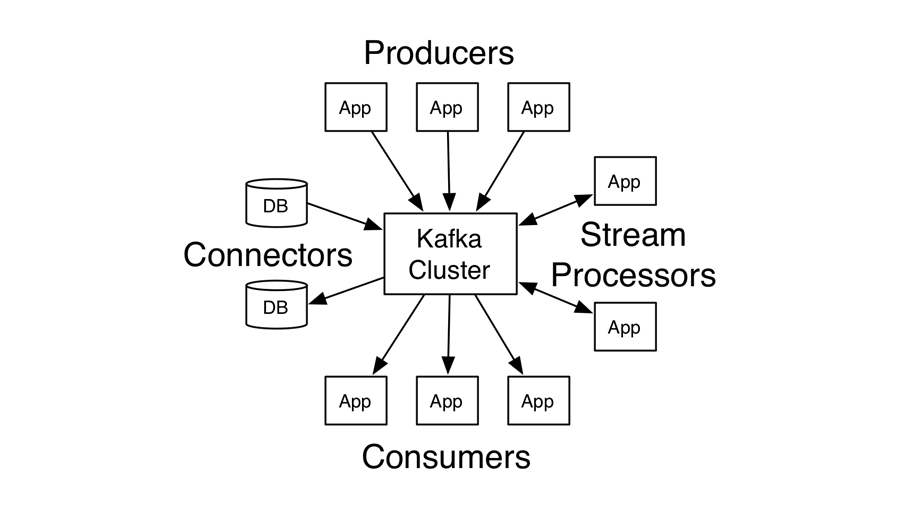
\includegraphics[width=\textwidth]{images/kafka.png}\\
%   \caption{Illustrazione di un sistema a servizi con Apache Kafka}
%   \captionsetup{aboveskip=2pt,font=it}
%   \caption*{Fonte: https://kafka.apache.org/20/documentation.html}
% \end{figure}
%
% Kafka è una piattaforma di \textit{event streaming}, un sistema moderno e distribuito basato sugli eventi anzichè su di una soluzione più classica come può essere quella del \textit{request/response}.
% L'adozione del \software\ nell'ambito dell'EAI è in crescita dato le dimostrate qualità nel gestire grandi moli di dati: la sua performance, sicurezza e scalabilità sono i punti che hanno portato il software al suo attuale successo.
%
% % \bigskip\noindent
% % Esposizioni delle ragioni personali che hanno portato alla scelta di tale percorso.


\subsection{Kafka come Middleware}

Per soddisfare le esigenze di innovazione l'azienda ha avviato un percorso per indagare le capacità del software Apache Kafka nell'ambito dell'integrazione aziendale.

\bigskip
\begin{figure}[h]
  \begin{center}
    
\includegraphics[width=0.14\textwidth]{images/kafka_logo.png}
    \caption{Logo di Apache Kafka}
    \captionsetup{aboveskip=2pt}
    \caption*{\begin{footnotesize}\textit{Fonte:} \url{https://commons.wikimedia.org/wiki/File:Apache_kafka.svg}\end{footnotesize}}
  \end{center}
\end{figure}

Kafka è una piattaforma di \textit{event streaming}, un sistema distribuito e moderno basato sugli eventi anzichè su di una soluzione più classica come può essere quella del \textit{request/response}.
Apache Kafka si integra ottimamente in molti sistemi basati sulle Architetture a messaggio, in cui lo scambio affidabile di dati in tempo reale è essenziale.

Il \software\ ha dimostrato negli anni recenti un notevole successo in diversi campi\footnote{Fonte: \url{https://kafka.apache.org/powered-by}}, come quello del flusso di \textit{Big Data}, del monitoraggio e dell'elaborazione dati in tempo reale.
L'adozione del \software\ nell'ambito dell'EAI è in crescita dato le dimostrate qualità nel gestire grandi moli di dati: la sua performance, sicurezza e scalabilità sono i punti che hanno portato il software al suo attuale successo.

L'interesse di Sync Lab nel \software\ risiede dunque nell'utilizzo di Kafka come un  \textit{Middleware} per soddisfare i problemi di integrazione aziendale e reingegnerizzare i flussi di dati preesistenti, ovvero sviluppare un nuovo sistema che consenta la comunicazione tra differenti servizi con un rapido flusso di dati fra di essi.


\bigskip
\begin{figure}[h]
  \begin{center}
    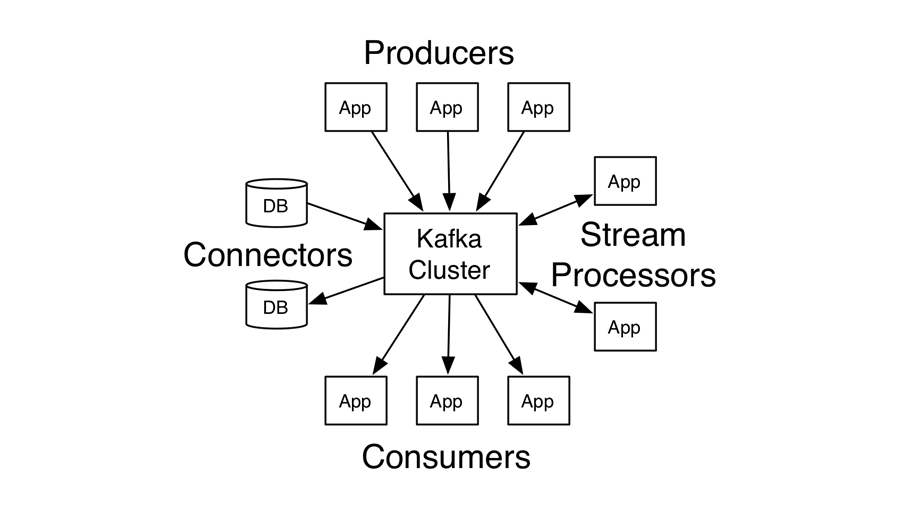
\includegraphics[width=0.8\textwidth]{images/kafka.png}
    \caption{Illustrazione di un sistema a servizi con Kafka}
    \captionsetup{aboveskip=2pt}
    \caption*{\begin{footnotesize}\textit{Fonte:} \url{https://kafka.apache.org/20/documentation.html}\end{footnotesize}}
  \end{center}
\end{figure}


L'azienda ha avviato un percorso per testare le capacità di Kafka rispetto agli attuali strumenti utilizzati nel settore, per valutare i vantaggi e svantaggi che l'adozione di tale \software\ può fornire al cliente.

\bigskip\noindent
Sono numerosi i vantaggi che Kafka può portare nel settore, fra cui:
\begin{itemize}
  \item gestione rapida e performante di un enorme flusso di dati;
  \item scalabilità;
  \item sicurezza riguardo la persistenza dei dati;
  \item semplice integrazione e affiancamento a sistemi già esistenti;
  \item l'essere una piattaforma \textit{open source};
  \item processazione dei dati in tempo reale integrata.
\end{itemize}

% \bigskip\noindent
% TODO: Come Kafka possa risolvere i problemi e le necessità viste qui sopra.

\section{Motivazioni e obiettivi personali}

\subsection{Scelta del percorso}

Una delle ragioni che mi ha portato a scegliere questo percorso di \stage\ è l'interesse verso Apache Kafka.
L'utilizzo della piattaforma di \textit{event streaming} è sempre più in crescita, come l'evoluzione verso sistemi sempre più distribuiti e a microservizi.

Un altro fattore fondamentale alla scelta del percorso sono stati la famigliarità con l'azienda, il personale giudizio positivo che ho avuto riguardo il loro metodo di lavoro e la libertà di sviluppo concessa: ho ritenuto importante la possibilità di elaborare personalmente un'architettura del caso d'uso con una visione ad alto livello, anzichè il semplice sviluppo di un software predeterminato e dal percorso strettamente imposto.

\subsection{Obiettivi personali}
L'obiettivo fondamentale dello \stage\ è colmare il divario tra il mondo accademico e quello lavorativo.
Grazie al percorso di \stage\ in una ditta esterna ho avuto l'opportunità di conoscere l'ambiente di lavoro di un'azienda nel campo \sacr{ict}, facilitandomi l'inserimento nel mondo del lavoro.

Un altro obiettivo è ottenere una formazione riguardo la tecnologia di Kafka, che ritengo possa arricchire fortemente le mie capacità e \textit{skill} professionali.
Sono pertanto interessato a sviluppare la mia formazione riguardo l'utilizzo e le implicazioni di questa tecnologia in rapida espansione, la cui formazione potrà essermi utile in molti campi anche al di fuori degli obiettivi dell'azienda ospitante lo \stage.


\section{Il percorso di Stage}


% Descrizione di come il percorso di \textit{stage} si inserisce nella visione più ampia riportata qui sopra.
%
% \bigskip\noindent
% Elenco degli obiettivi del percorso:
% \begin{itemize}
%   \item formazione riguardo Kafka e l’ambito dell’integrazione;
%   \item verificare le capacità di Kafka nell’ambito EAI;
%   \item sperimentare l’utilizzo di Kafka come \textit{Middleware} tramite una simulazione di un caso d’uso reale a servizi indipendenti.
% \end{itemize}
%
% \noindent
% Breve esposizione dei motivi che mi hanno portato a scegliere questo percorso

% TODO:
% - motivazioni riguardo il percorso di stage proposto
% - descrizione del percorso di stage tenendo conto del contesto e degli obiettivi citati sopra
% - descrivere i miei obiettivi rispetto a quelli aziendali
\subsection{Obiettivi dello \textit{stage}}

Il percorso di \textit{stage} offerto dall'azienda si inserisce all'interno della strategia aziendale più ampia descritta sopra.
Al fine di esplorare la tecnologia di Apache Kafka nell'ambito di un \textit{Middleware} per l'integrazione aziendale, l'azienda ha proposto un percorso di \textbf{\textit{stage} il cui obiettivo è la reingegnerizzazione di un flusso di dati asincrono, utilizzando un'architettura basata su Kafka all'interno di un caso d'uso simulato tramite servizi indipendenti.}

\bigskip
Lo stagista ha il compito di osservare, testare e verificare che il \software\ possa svolgere alcuni compiti inerenti all'area del \sacr{eai}, analizzando alcuni casi d'uso presenti in un \textit{Middleware} aziendale in ambito \textit{telco}.
Il percorso di prevede una durata di 300 ore lavorative.

% \bigskip\noindent
% Il percorso proposto prevede le seguenti attività e obiettivi generali:
% \begin{itemize}
%   \item formazione riguardo la piattaforma di \textit{event streaming} Kafka e l'ambito dell'integrazione aziendale;
%   \item verifica delle capacità di Kafka nell'EAI;
%   \item sperimentazione e sviluppo di un \textit{Middleware} basato su Kafka tramite una simulazione di un caso d'uso reale a servizi indipendenti.
% \end{itemize}

\subsection{Prodotti attesi}

I prodotti attesi al termine dello \textit{stage} sono dunque associati alla realizzazione di tre flussi di integrazione, basati su dei casi d’uso reali, per la gestione dei paradigmi di integrazione asincrono e asincrono con \textit{callback} (due requisiti obbligatori), e sincrono ove fosse disponibile del tempo aggiuntivo e se ritenuto opportuno; durante il percorso considerato il contesto e le opportunità offerte dal \software\ questo obiettivo verrà sostituito per testare delle funzionalità aggiuntive di Kafka.

\subsection{Contenuti formativi previsti}

La realizzazione di questi prodotti necessita una sostanziale formazione dello stagista riguardo i principali concetti del settore del \textit{Enterprise Application Integration} e l'utilizzo della piattaforma di \textit{event streaming} Kafka.
Più precisamente, i contenuti formativi previsti durante questo percorso di \textit{stage} sono i seguenti:
\begin{itemize}
  \item Concetti chiave del \gls{g_eai};
  \item \textit{Design archittetturali};
  \item Cenni di \textit{Networking} applicato alle architetture distribuite;
  \item Architetture di Integrazione e \textit{Middleware};
  \item Apache Kafka.
\end{itemize}

\subsection{Interazione tra studente e referenti aziendali}
% Personalizzare definendo le modalità di interazione col tutor aziendale
Regolarmente, (almeno una volta la settimana) ci saranno incontri online (tramite la piattaforma Google Meet) con il tutor aziendale Francesco Giovanni Sanges, il responsabile dell’area \sacr{eai} Salvatore Dore e gli esperti delle tecnologie affrontate.
I meeting saranno necessariamente online, dato il dislocamento dei vari membri in diverse città.

Lo scopo di questi incontri sarà quello di verificare lo stato di avanzamento, chiarire gli obiettivi ove necessario, affinare la ricerca e aggiornare la pianificazione iniziale.

\subsection{Pianificazione del lavoro}

Ad ogni incremento è associato un requisito obbligatorio, desiderabile o facoltativo.
A questi requisiti vi è associato un codice identificativo per favorirne il tracciamento futuro, in che precede la voce descrittiva dell'incremento.
\noindent
Ogni codice è composto da una lettera seguita da dei numeri interi, secondo il seguente modello:
\begin{center}
	\textbf{A-X.Y.Z}
\end{center}
ove, da sinistra verso destra:
\begin{itemize}

  \item \textbf{A} rappresenta la lettera che qualifica il requisito come obbligatorio, desiderabile o facoltativo, secondo la seguente notazione:
  \begin{itemize}
  	\item \textit{O} per i requisiti obbligatori, vincolanti in quanto obiettivo primario richiesto dal committente;
  	\item \textit{D} per i requisiti desiderabili, non vincolanti o strettamente necessari,
  		  ma dal riconoscibile valore aggiunto;
  	\item \textit{F} per i requisiti facoltativi, rappresentanti valore aggiunto non strettamente
  		  competitivo.
  \end{itemize}

  \item \textbf{X} rappresenta la settimana in cui viene inizialmente pianificato l'incremento (identificata da un numero incrementale e intero, partendo da 1).
  Questo consente allo studente, al tutor interno e al tutor interno una rapida quantificazione dell'avanzamento corrente dello stage rispetto a quanto inizialmente pianificato.

  \item \textbf{Y} rappresenta la posizione sequenziale prevista dell’incremento all’interno della settimana (incrementale e intero, partendo da 1). Esso è strettamente associato alla lettera.


\end{itemize}
\noindent
Di seguito viene presentata la pianificazione settimanale delle ore lavorative previste.
Ad ogni settimana sono assegnate le voci contenenti gli incrementi previsti in essa, ove i codici utilizzano la notazione descritta precedentemente.

\begin{itemize}
       \item \textbf{Prima Settimana (40 ore)}
       \begin{itemize}
           \item \textbf{O-1.1} Incontro con le persone coinvolte nel progetto per discutere i requisiti e le richieste relative al sistema da sviluppare;
           \item \textbf{O-1.2} Verifica credenziali e strumenti di lavoro assegnati;
           \item \textbf{O-1.3} Presa visione dell’infrastruttura esistente;
           \item \textbf{D-1.1} Ripasso approfondito riguardo i seguenti argomenti:
             \begin{itemize}
               \item Ingegneria del \software;
               \item Sistemi di versionamento;
               \item Architetture \software;
               \item Cenni di \textit{Networking}.
             \end{itemize}
       \end{itemize}

       \item \textbf{Seconda Settimana (40 ore)}
       \begin{itemize}
           \item \textbf{O-2.1} Nozioni fondamentali riguardo \sacr{eai} e \sacrfoot{soa};
           \item \textbf{O-2.2} Approfondimenti riguardo le Architetture a Messaggio, in particolare:
             \begin{itemize}
               \item \textit{Integration Styles};
               \item \textit{Channel Patterns};
               \item \textit{Message Construction Patterns};
               \item \textit{Routing Patterns};
               \item \textit{Transformation Patterns};
               \item \textit{System Management Patterns}.
             \end{itemize}
       \end{itemize}

       \item \textbf{Terza Settimana (40 ore)}
       \begin{itemize}
           \item \textbf{O-3.1} Apache Kafka:
             \begin{itemize}
               \item Introduzione a Kafka;
               \item Concetti fondamentali di Kafka;
               \item Avvio e \sacrfoot{cli};
               \item Programmazione in Kafka con Java.
             \end{itemize}
           \item \textbf{D-3.1} Esempi e applicazioni di Apache Kafka.
       \end{itemize}


       \item \textbf{Quarta Settimana (40 ore)}
       \begin{itemize}
           \item \textbf{O-4.1} Confluent Platform:
             \begin{itemize}
               \item Service registry;
               \item REST proxy;
               \item kSQL;
               \item Confluent connectors;
               \item Control center.
             \end{itemize}
       \end{itemize}

       \item \textbf{Quinta Settimana (40 ore)}
       \begin{itemize}
         \item \textbf{O-5.1} Analisi dei casi d'uso reali;
         \item \textbf{O-5.2} Realizzazione dei componenti per l'esecuzione dei casi di test.
       \end{itemize}

       \item \textbf{Sesta Settimana (40 ore)}
       \begin{itemize}
         \item \textbf{O-6.1} Analisi reingegnerizzazione e collaudo del flusso di integrazione asincrono.
       \end{itemize}

       \item \textbf{Settima Settimana (40 ore)}
       \begin{itemize}
           \item \textbf{O-7.1} Analisi e reingegnerizzazione e collaudo del flusso di integrazione asincrono con callback

       \end{itemize}

       \item \textbf{Ottava Settimana (20 ore)}
       \begin{itemize}
           \item \textbf{D-8.1} Analisi e reingegnerizzazione e collaudo del flusso di integrazione sincrono.
       \end{itemize}

\end{itemize}
\clearpage\noindent
Secondo questa pianificazione, le 300 ore di \stage\ previste sono approsimativamente divise in:
\begin{itemize}
  \item 160 ore di Formazione sulle tecnologie;
  \item 60 ore di Progettazione dei componenti e dei test;
  \item 60 ore di Sviluppo dei componenti e dei test;
  \item 20 ore di Valutazioni finali, Collaudo e Presentazione della Demo.
\end{itemize}
